\highlight{
  The dependency quantity analysis 
is performed on basis of an improved version of control flow graph of the program, called abstract control flow graph.
In this part, I first show how to generate this abstract execution control flow graph in Section~\ref{sec:static-abscfg}
Then in Section~\ref{sec:static-reachability}, 
I present a reachability-bound analysis algorithm adapted from the newly-designed
technique in Chapter~\ref{sec:reachability-analysis} for estimating the reaching times of every program location.
Section~\ref{sec:static-quantity-node}
uses the reachability-bound analysis results estimating the dependency quantity
over labeled variable and
Section~\ref{sec:static-quantity-edge} uses the same information
estimating the dependency quantity for the pairs of dependent variables.
In Appendix~\ref{apdx:reachability_soundness},
this static algorithm is proved as the sound approximation of the dependency quantity
from the execution-based analysis in Section~\ref{sec:dynamic-reachability}.
%  before the introduction of  the edge and weight estimation.  
}
\highlight{
  Previous static analysis doesn't have analysis on the quantitative property.
  Comparing to it, the new technique on estimating the quantity property helps to improve the adaptivity estimation.
}
\subsubsection{Abstract Execution Control Flow graph}
\label{sec:static-abscfg}

% I discuss the vertices and edge of the
% abstract control flow graph for a program $c$, $\absG(c)$.
% In the abstract control flow graph,
% every 
% vertex corresponds to the unique
% label.
The abstract control flow graph is a control flow graph, with annotations on every edge. It is constructed as follows.
\paragraph*{Vertices of Abstract Control Flow Graph}
The abstract control flow graph enriches the standard control flow graph vertices set with
one extra label, $l_{lex}$ for each program $c$.
Specifically,
the vertices of this graph is the set of $c$'s labels with an exit label $l_{ex}$, 
\[ 
  \absV(c) = labels(c)\cup\{l_{ex}\}
\]
%  corresponding to a label command in the program.

Overall, the vertices can be easily collected and the key point of construction of the abstract execution control flow graph for a program is the abstract execution trace, 
which relies on the abstraction of expression and abstract transition (we also call it abstract event), I will discuss in the following section.

\paragraph*{Edges of Abstract Control Flow Graph}
  The edge in the abstract control flow graph comes from the abstract execution trace of the program. 
  The abstract execution trace, an abstract representation of the execution, consists of a list of abstract transitions. 
  Then, every abstract transition in the abstraction execution trace corresponds to an edge in the abstract control flow graph.
  In another word, the edge $(l_1, dc, l_2)$ in the abstract control flow graph, represents an abstract transition 
 from $l_1$ to $l_2$, with a set of difference constraints $dc$. 
 Also notice, the difference constraints generated during the abstract transition appears in the edge as annotation.
% \wq{
  %  To make it easy to understand, 
  % }  
%
\paragraph{Edge Construction Step 1: Expression Abstraction}

The expression assigned to the variable on the left hand of the assignment command is abstracted to an abstract value: (adopted from the expression abstraction method in paper \cite{sinn2017complexity}). The abstract value is expressed in the form of Difference constraint, denotated as $DC : \mathcal{VAR} \cup \constdom \to \mathcal{\mathcal{VAR} \times (\mathcal{VAR} \cup \constdom) } \times (\mathbb{Z} \cup \{\infty\})$.  $\constdom$ is called the Symbolic Constant defined as $\constdom \triangleq \mathbb{N} \cup \inpvar \cup \{\max{(\dbdom)}\} $, which consists of 
natural numbers $\mathbb{N}$,
the program's input variables $\inpvar$  
and a constant value $\max(\dbdom)$ for estimating the upper bound of variables which are
assigned by queries. 

Give an instance of difference constraint used here,
$DC(\mathcal{VAR}  \cup \constdom) \cup \{\top\}$ represents all the difference constraints over 
variable and symbolic constants. 
% The difference constraint $DC$ over $\mathcal{VAR} \cup \constdom$ 
It is a set of the inequality of form $x \leq y + v$ where $x \in \mathcal{VAR} $, 
$y \in \mathcal{VAR}  \cup \constdom$ and $v \in \mathbb{Z}$. 
This difference constraint is defined in the same way as
\cite{sinn2017complexity}. For concise, I use $\dcdom^{\top}$ to represent the $DC(\mathcal{VAR}  \cup \constdom) \cup \{\top\}$ .


 I show the expression abstraction $\absexpr : \expr \to \mathcal{VAR} \to DC(\mathcal{VAR}  \cup \constdom) \cup \{\top\} $ below.

%  I introduce the following notations and operations first
% % an expression abstraction method based on the expression abstraction in paper \cite{sinn2017complexity}.
% \\
% % is enriched into $\constdom \triangleq \mathbb{N} \cup \inpvar \cup \{\max{(\dbdom)}\} $.
% T
% \\

% represents the set of inequality over all $\mathcal{VAR}  \cup \constdom$. 

% The symbolic constant is enriched into $\constdom \triangleq \mathbb{N} \cup \inpvar \cup \{\max{(\dbdom)}\} $.
% It consists of 
% natural number $\mathbb{N}$,
% the symbolic constants $\inpvar$ (i.e., the set of the program's input variables), 
% and a constant value $\max(\dbdom)$ for estimating the upper bound of variables which are
% assigned by queries.
% \\
% The symbolic constant is enriched into $\constdom \triangleq \mathbb{N} \cup \inpvar \cup \{\max{(\dbdom)}\} $.
% \\

% % $ \absdom: \mathcal{P}(DC(\mathcal{VAR}  \cup \constdom) \cup \{\top \})$:
% \\
% $\constdom: \mathbb{N} \cup \inpvar \cup \{\max{(\dbdom)}\} $ 
% The  constant 
% \\
% % $DC(\mathcal{VAR}  \cup \constdom)$ represents the set of inequality over all $\mathcal{VAR}  \cup \constdom$.
% \\

% \[
%   \begin{array}{ll} 
%     \absexpr(y + c, x)  = x' \leq y + c  & c \in \mathbb{N} \land y \in (VAR \cup \constdom) \\
%     \absexpr(y - c, x)  = x' \leq y - c  & c \in \mathbb{N} \land y \in (VAR \cup \constdom) \\
%     \absexpr(v, x)  = x' \leq v + 0  & v \in (VAR \cup \constdom) \\
%     \absexpr(\aexpr, x) = x' \leq 0 + \infty   & \aexpr \text{ doesn't have any of the forms as above} \\
%     \absexpr(\qexpr, x)  = x' \leq 0 + \max(\dbdom) & \qexpr \text{ is a query expression}  \\
%     \absexpr(\bexpr, x) = x' \leq 0 + 1   & \bexpr \text{ is a boolean expression} \\
%   \end{array}
%   \]
  \[
    \begin{array}{ll} 
      \absexpr(x - v, x)  = x' \leq x - v  & x \in \grdvar \land v \in \mathbb{N} \\
      \absexpr(y + v, x)  = x' \leq y + v  & x \in \grdvar \land v \in \mathbb{Z} \land y \in (\grdvar \cup \constdom) \\
      \absexpr(v, x)  = x' \leq v + 0  & x \in \grdvar \land v \in (\grdvar \cup \constdom) \\
      \absexpr(y + v, x)  = x' \leq y + v & \\
      \grdvar = \grdvar \cup \{y\} & x \in \grdvar \land v \in \mathbb{Z} \land y \notin (\grdvar \cup \constdom)  \\
      \absexpr(\qexpr, x)  = x' \leq 0 + \max(\dbdom) & x \in \grdvar \land \qexpr \text{ is a query expression}  \\
      \absexpr(\bexpr, x) = x' \leq 0 + 1   & x \in \grdvar \land \bexpr \text{ is a boolean expression} \\
      \absexpr(\expr, x) = x' \leq \infty  &  x \in \grdvar \land \expr \text{ doesn't have any of the forms as above} \\
      \absexpr(\expr, x) = \top  &  x \notin \grdvar \\
    \end{array}
    \]
  
  % \wq{ 
    $\grdvar$ is the set of variables used in the guard expression of every while command in the program $c$. 
  % }. 
  In the case 4, if a variable $x$, belonging to the set 
  $\grdvar$ is updated by a variable $y$, which isn't in this set, 
  I add $y$ into the set $\grdvar$ and repeat 
  above procedure  until $\grdvar$ and $\absexpr(\expr, x)$ is stabilized. 
  % \wq{I do not understand this sentence:-(}
  \\
Specifically 
% understanding the intuition, 
we handle a 
% simplified 
normalized guard expression ($ x > 0$ for $x^l \in \lvar_c$)
 in $\ewhile$, and 
%  \wq{I do not understand this sentence:-(}
%  .
% \\
% The counter variables only increase, decrease or reset by expression in the form of arithmetic minus and plus (able to extend to max and min.)
the counter variables only increase, decrease or reset by 
% expression in the form of 
simple arithmetic expression (mainly multiplication, division, minus and plus (able to extend to max and min)). 
This is the same as in paper \cite{sinn2017complexity}. 
\\
For more complex expression assignments, where the counter reset, or calculated from $\elog$, 
multiplication or division, and expressions involving multiple variables, the constraint is approximated as reset of $\infty$.
\\
% This simplification \wq{which part I simplify here?} 
This approximation strategy
doesn't affect our analysis results in our examples. It is easy to extend the normalized expression 
into more complex forms as in \cite{sinn2017complexity}, as well as the 
counter variable manipulation with more advanced expressions.
% \\ 
% The boolean expression in the guard of $\ewhile$ command is normalized into form of $ x > 0$ where $x^l \in \lvar_c$ for some $l$.

\paragraph{Edge Construction Step 2: Abstract Initial and Final State}
%
Abstract initial state: $\absinit(c) \in \ldom$,
Abstract Final State: $\absfinal(c) \in \mathcal{P}(\ldom \times \dcdom^{\top})$

The \emph{Abstract initial state} for a program $c$ is the initial label of this program.
This label corresponds to the first labeled command of this program 
when executing this program.
\\
Given a program $c$, its abstract initial state is computed as follows,
%
\[
  \begin{array}{ll}
    \absinit(\clabel{\assign{x}{\expr}}{}^l)  & = l  \\
    \absinit(\clabel{\assign{x}{\query(\qexpr)}}{}^l)  & = l \\
    \absinit(\clabel{\eskip}^{l})  & = l \\
    \absinit(\eif [b]^l \ethen c_1 \eelse c_2)  & = l \\
    \absinit(\ewhile [b]^l \edo c)  & = l \\
    \absinit(c_1 ; c_2)  & = \absinit(c_1) \\
 \end{array}
 \]
%

The \emph{Abstract Final State} of the program $c$, 
$\absfinal(c) \in \mathcal{P}(\ldom \times \dcdom^{\top})$
is a set of pairs, with a label as first component and a constraint as the second component.
Every pair in $\absfinal(c)$ corresponds to a labeled command of $c$,
and the constraint in this pair is computed by $\absexpr$ in the first step.
\\
Given a program $c$, its final state is computed as follows,
$\absfinal: \cdom \to \mathcal{P}(\ldom \times \dcdom^{\top})$,
% computes the set of Abstract Final State for the command. 
 \[
  \begin{array}{ll}
    \absfinal(\clabel{\assign{x}{\expr}}{}^l)  & = \{(l, \absexpr\eapp (\expr, x))\}  \\
     \absfinal(\clabel{\assign{x}{\query(\qexpr)}}{}^l)  & = \{
      (l, x' \leq 0 + Q_m )\}  \\
     \absfinal(\clabel{\eskip}^{l})  
     & = \{(l, \top)\} \\
     \absfinal(\eif [b]^l \ethen c_1 \eelse c_2)  & = \absfinal(c_1) \cup \absfinal(c_2) \\
     \absfinal(\ewhile [b]^l \edo c)  & = \{(l, \absexpr(\bexpr, \top))\} \\
     \absfinal(c_1 ; c_2)  & =  \absfinal(c_2) \\
 \end{array}
 \]

% \paragraph{Edge Construction Step 3: Program Event Abstraction}
%  I show the abstract event definition, which is generated when computing its abstract execution trace.

% \begin{defn}[Abstract Event]
%   \label{def:abs_event}
%   Abstract Event: 
%   $\absevent \in $
%   $\ldom \times \dcdom^{\top} \times \ldom$
%   is a 
%   % pair of abstract initial state and final state.
%   triple where the first and third components are labels,
%   second component is a constraint from $\dcdom^{\top}$.
%   % the thrid % computed from program's abstract final and initial state, $\absfinal(c)$ and $\absinit(c)$ with formal definition, and algorithm detail in Appendix.
%   %  the constraint and the third corresponds to a final state.
%   \end{defn}
%   Specifically, in an abstract event, 
%   the first label correspond to an initial state, and 
%   the second label and the constraint correspond to an abstract final state.
%  The abstract initial state is a label from $\ldom$.
% The abstract final state is a pair from $\ldom \times \dcdom^{\top}$,  
% where first component is a label from $\ldom$ and the second component is a constraint from $\dcdom^{\top}$.
% %

% %
% Given a program $c$, its abstract initial state,
% and the set of its abstract final state is computed as follows,
% %
% \[
%   \begin{array}{ll}
%     \absinit(\clabel{\assign{x}{\expr}}{}^l)  & = l  \\
%     \absinit(\clabel{\assign{x}{\expr}}{}^l)  & = l \\
%     \absinit(\clabel{\eskip}^{l})  & = l \\
%     \absinit(\eif [b]^l \ethen c_1 \eelse c_2)  & = l \\
%     \absinit(\ewhile [b]^l \edo c)  & = l \\
%     \absinit(c_1 ; c_2)  & = \absinit(c_1) \\
%  \end{array}
%  \]
% %
% Final State Abstraction: 
% $\absfinal: \cdom \to \mathcal{P}(\ldom \times \dcdom^{\top})$,
% computes the set of Abstract Final State for the command. 
%  \[
%   \begin{array}{ll}
%     \absfinal(\clabel{\assign{x}{\expr}}{}^l)  & = \{(l, \absexpr\eapp (\expr, x))\}  \\
%      \absfinal(\clabel{\assign{x}{\query(\qexpr)}}{}^l)  & = \{
%       (l, x' \leq 0 + \max(\dbdom) )\}  \\
%      \absfinal(\clabel{\eskip}^{l})  
%      & = \{(l, \top)\} \\
%      \absfinal(\eif [b]^l \ethen c_1 \eelse c_2)  & = \absfinal(c_1) \cup \absfinal(c_2) \\
%      \absfinal(\ewhile [b]^l \edo c)  & = \{(l, \top)\} \\
%      \absfinal(c_1 ; c_2)  & =  \absfinal(c_2) \\
%  \end{array}
%  \]
%  %
%  \paragraph{Edge Construction Step 3: Abstract Execution Trace Generation}
%  Now, I  extract the abstract execution trace  $\absflow(c)$ for a program, which computes the Abstract Execution Trace for program $c$, as a set of the abstract events $\absevent$.
%  %
%  \begin{defn}[Abstract Execution Trace]
%  \label{def:abs_trace}
%   $\absflow \in \cdom \to \mathcal{P}( \ldom \times DC(\mathcal{VAR}  \cup \constdom) \cup \{\top\}) \times \ldom )$
%   \end{defn}
%  %

 
%    I now show how to compute the abstract execution trace. 
%   For simplicity, I use $\mathcal{P}(\absevent)$ represent the power set of all abstract events, and I have $\absflow(c) \in \mathcal{P}(\absevent)$.
%   I first append a skip command with 
% %  a symbolic label $l_e$, i.e., $\clabel{\eskip}^{l_e}$ at the end of the program $c$, and compute the $\absflow(c) = \absflow'(c')$ for $c'$, where $c' = c;\clabel{\eskip}^{l_e}$ as follows,
% the exist label $l_{ex}$, i.e., $\clabel{\eskip}^{l_{ex}}$ at the end of the program $c$, 
% and compute the $\absflow(c) = \absflow'(c')$ for $c'$, where $c' = c;\clabel{\eskip}^{l_{ex}}$ as follows,
%  %
\paragraph{Abstract Event and Execution Trace} 
 \emph{Abstract Event}: 
   $\absevent \in $
   $\ldom \times \dcdom^{\top} \times \ldom$,
  \emph{Abstract Execution Trace}: $\absflow \in \cdom \to \mathcal{P}( \ldom \times \dcdom^{\top} \times \ldom )$

 The abstract event is generated during computing its abstract execution trace, its type is defined as follows,
 \begin{defn}[Abstract Event]
   \label{def:abs_event}
   Abstract Event: 
   $\absevent \in $
   $\ldom \times \dcdom^{\top} \times \ldom$
   is a 
   % pair of abstract initial state and final state.
   triple where the first and third components are labels,
   second component is a constraint from $\dcdom^{\top}$.
   % the thrid % computed from program's abstract final and initial state, $\absfinal(c)$ and $\absinit(c)$ with formal definition, and algorithm detail in Appendix.
   %  the constraint and the third corresponds to a final state.
   \end{defn}
   Specifically, in an abstract event, 
   the first label correspond to an initial state, and 
   the second label and the constraint correspond to an abstract final state.
  The abstract initial state is a label from $\ldom$.
 The abstract final state is a pair from $\ldom \times \dcdom^{\top}$,  
 where first component is a label from $\ldom$ and the second component is a constraint from $\dcdom^{\top}$.
 %
 For simplicity, we use $\mathcal{P}(\absevent)$ represent the power set of all abstract events, and we have $\absflow(c) \in \mathcal{P}(\absevent)$.

%  Now, we  extract the abstract execution trace  $\absflow(c)$ for a program, which computes the 
 The \emph{Abstract Execution Trace} for program $c$ is a set of the abstract events $\absevent$.
 Its type is formally defined as follows in Definition~\ref{def:abs_trace}.
 %
 \begin{defn}[Abstract Execution Trace]
 \label{def:abs_trace}
  $\absflow \in \cdom \to \mathcal{P}( \ldom \times \dcdom^{\top} \times \ldom )$
  \end{defn}
 %
 The \emph{Abstract Execution Trace} for program $c$ is computed as follows.
 \\
  % We now show how to compute the abstract execution trace. 
 We first append a $\eskip$ command with 
%  a symbolic label $l_e$, i.e., $\clabel{\eskip}^{l_e}$ at the end of the program $c$, and compute the $\absflow(c) = \absflow'(c')$ for $c'$, where $c' = c;\clabel{\eskip}^{l_e}$ as follows,
the label $\lex$, i.e., $\clabel{\eskip}^{l_{ex}}$ at the end of the program $c$, and construct 
the program $c' = c;\clabel{\eskip}^{l_{ex}}$.
Then, we compute the $\absflow(c) = \absflow'(c')$ for $c'$ as follows,
 {\footnotesize
 \[
   \begin{array}{ll}
      \absflow'(\clabel{\assign{x}{\expr}}{}^l)  & = \emptyset  \\
      \absflow'(\clabel{\assign{x}{\query(\qexpr)}}{}^l)  & = \emptyset  \\
      \absflow'([\eskip]^{l})  & = \emptyset \\
      \absflow'(\eif [b]^l \ethen c_t \eelse c_f)  & =  \absflow'(c_t) \cup \absflow'(c_f)
      %   \\ & \quad 
        \cup \{(l, \top,  \absinit(c_t) ) ,  (l, \top, \absinit(c_f)) \} \\
       \absflow'(\ewhile [b]^l \edo c_w)  & =  \absflow'(c_w) \cup \{(l, \top, \absinit(c_w)) \} 
      %  \\ & \quad 
       \cup \{(l', dc, l)| (l', dc) \in \absfinal(c_w) \} \\
       \absflow'(c_1 ; c_2)  & = \absflow'(c_1) \cup  \absflow'(c_2) 
      %  \\ & \quad 
       \cup \{ (l, dc, \absinit(c_2)) | (l, dc) \in \absfinal(c_1) \} \\
   \end{array}
   \]
   }

   Notice $\absflow'([x := \expr]^{l})$, $\absflow'([x := \query(\qexpr)]^{l})$ and $\absflow'([\eskip]^{l})$ are all empty set. 
   For every event $\event$ with label $l$ in an execution trace $\trace$ of program $c$, 
   there is an abstract event in program's abstract execution trace of form $(l, \_, \_)$.  
    I also show the soundness of the abstract execution trace in Appendix.
  %  which says 
  %  \wq{...}
   \begin{lem}[Soundness of the Abstract Execution Trace]
     \label{lem:abscfg_sound}
   Given a program ${c}$, I have:
   %
   \[
     \begin{array}{l}
       \forall \vtrace_0, \trace \in \mathcal{T} ,  \event = (\_, l, \_) \in \eventset \sthat 
   \config{{c}, \trace_0} \to^{*} \config{\eskip, \trace_0 \tracecat \vtrace} 
   \land \event \in \trace 
   \\
   \qquad \implies \exists \absevent = (l, \_, \_) \in (\ldom\times \dcdom^{\top} \times \ldom) \sthat  
   \absevent \in \absflow(c)
   \end{array}
   \]
   \end{lem}
%    This lemma is proved formally in Appendix~\ref{apdx:reachability_soundness}.
% For every event $\event$ with label $l$ in an execution trace $\trace$ of program $c$, 
% there is an abstract event in program's abstract execution trace of form $(l, \_, \_)$. 
This lemma is proved formally in Lemma~\ref{lem:abscfg_sound} in Appendix~\ref{apdx:reachability_soundness}.
\\
For every labeled variable in program $c$, $x^l \in \lvar_c$, there is a unique abstract event in program's abstract execution trace $\absevent \in \absflow(c)$ of form $(l, \_, \_)$. 
\begin{lem}[Uniqueness of the Abstract Execution Trace]
  \label{lem:abscfg_unique}
Given a program ${c}$, I have:
%
\[
  \begin{array}{l}
    \forall \vtrace_0, \trace \in \mathcal{T} ,  \event = (\_, l, \_, \_) \in \eventset^{\asn} \sthat 
\config{{c}, \trace_0} \to^{*} \config{\eskip, \trace_0 \tracecat \vtrace} 
\land \event \in \trace 
\\
\qquad \implies \exists! \absevent = (l, \_, \_) \in (\ldom\times \dcdom^{\top} \times \ldom) \sthat  
\absevent \in \absflow(c)
\end{array}
\]
\end{lem}
This lemma and proof is also 
formalized in Lemma~\ref{lem:absevent_unique} in Appendix~\ref{apdx:reachability_soundness}.

Then, I build the edge for $c$'s abstract control flow graph as follows,
\[
  \absE(c) = \{(l_1, dc, l_2) | (l_1, dc, l_2) \in \absflow(c)\}
  \]

%  I have a pre-processing algorithm to go through the programs and returns the list of labels associating with a loop and whose visiting times need to be analyzed.
%


\paragraph{Abstract Control Flow Graph} 
With the vertices $\absV(c)$ and edges $\absE(c)$ ready, I construct the abstract control flow graph, formally 
% Through a program $c$'s abstract execution trace, its abstract control flow graph is computed 
defined in 
Definition~\ref{def:abs_cfg}.
% Given program $c$ with its abstract control flow $\absflow(c)$, the Abstract Control Flow Graph:
% \\
\begin{defn}[Abstract Control Flow Graph]
\label{def:abs_cfg}
Given a program $c$, 
with its abstract control flow $\absflow(c)$
its abstract control flow graph $\absG(c) =(\absV(c), \absE(c), \absW(c))$ is defined as follows,
\\
% \highlight{
% :
%
% \\
$\absE(c) = \{(l_1, dc, l_2) | (l_1, dc, l_2) \in \absflow(c)\}$,
\\
$\absV(c) = labels(c)\cup\{l_{ex}\}$
\\
 $\absW(c) 
\triangleq \left\{ (l, w) \in \mathbb{L} \times EXPR(\constdom) \right\}$.
% }
% \\
% , where the weight of every label to be computed in the next step.
\end{defn}
% 
% The vertices $\absV(c)$ in this graph are program's labels with an exit label $l_{ex}$.
% Each directed 
%  edge $(l_1, dc, l_2)$ from $l_1$ to $l_2$,
%  represents an abstract transition 
%  between two control locations with a set of difference constraints on it.
% %  , i.e., the labels of two commands (we call the labels also control location and they refer to the same thing), 
% %  where 
% In this transition, the  command labeled with the second location $l_2$, 
%  will be executed after execution of the command with label $l_1$,
% %  The abstract transition contains a set of difference constraints for variables, 
% with the difference constraints generated by abstracting the command of the first label.
% % \\
% % It is easy to show for every $(l_1, dc, l_2) \in \absflow(c)$ such that $l_2 \neq l_e$, $(l_1, l_2) \in flow(c)$. The formal Lemma and proof can be found in Lemma~\ref{lem:flow_to_absflow} in Appendix~\ref{apdx:reachability_soundness}.
Notice I also define the $\absW(c)$ in this graph without giving an actual value.
This $\absW(c)$ is the set of weight for every 
% vertex 
label. The weight is a symbolic expression over the symbolic constant, 
which is the estimated upper bound on the number of visiting time for every control location
through the reachability bound analysis as follows.
%
% It is easy to show for every $(l_1, dc, l_2) \in \absflow(c)$ such that $l_2 \neq l_e$, $(l_1, l_2) \in flow(c)$. The formal Lemma and proof can be found in Lemma~\ref{lem:flow_to_absflow} in Appendix~\ref{apdx:reachability_soundness}.
%
\paragraph*{Abstract Control Flow Graph Through An Example}
%
\begin{example}[The Abstract Control Flow Graph for Two Rounds Data Analysis Program Example]
    For the same two adaptivity rounds example program, 
its generated abstract control flow graph is shown as in Figure~\ref{fig:abscfg_tworound}(b).
For example, the edge $(0, a \leq 0, 1)$ on the top, tells us the command 
$\clabel{\assign{a}{0}}^0$ is executed with next continuation location $1$,
where the 
command $\clabel{\assign{j}{k}}^1$ will be executed next.
The constraint $a \leq 0$ is a difference constraint, generated by abstracting from the assignment command $\assign{a}{0}$,
representing that value of $a$ is less than or equals to $0$ after 
location $0$ before executing command at line $1$. The difference constraint is an inequality relation between, the left-hand side of the inequality talks about the variable before the execution and the right-hand side ascribes those after the execution. 
Look at the $a < a+x $ on the edge $5$ to $2$, which describes the execution of the command at line $5$, which is an assignment $a = a+x$. The $a$ on the left side of $a < a+x$ represents the value of $a$ after the assignment, while the right-hand side $a$ stores the value before the assignment. 
Also, I have while loop, which is a circle $2 \to 4 \to 5 \to 2$ in Figure~\ref{fig:abscfg_tworound}(b). 
Please also look at the edge from $3$ to $4$, which talks about the query! The $x < \max(\dbdom)$ describes the execution of a query request (the command at line 3), the query results stored in $x$ is bounded by $\max(\dbdom)$. 
$\max(\dbdom)$ is the maximal value for query requesting result from the database $DB$. $top$ means there is no assignment executed, for example, I have the difference constraint $\top$ on the edge $2$ to $6$, means at line $2$, there is no assignment (it is a testing guard $j>0$.) 
%
The same way for the rest edges' constructions.
\begin{figure} 
  \centering
  \begin{subfigure}{.7\textwidth}
  \begin{centering}
  {\small
  $
      \begin{array}{l}
            \clabel{ \assign{a}{0}}^{0} ;   
              \clabel{\assign{j}{k} }^{1} ;\\
              \ewhile ~ \clabel{j > 0}^{2} ~ \edo ~ 
              \Big(
               \clabel{\assign{x}{\query(\chi[j])} }^{3}  ;
               \clabel{\assign{j}{j-1}}^{4} ;
              \clabel{\assign{a}{x + a}}^{5}       \Big);\\
              \clabel{\assign{l}{\query(\chi[k]*a)} }^{6}
          \end{array}
  $
  }
  \caption{}
  \end{centering}
  \end{subfigure}
    \begin{subfigure}{.45\textwidth}
    \begin{centering}
  %   \todo{abstract-cfg for two round}
  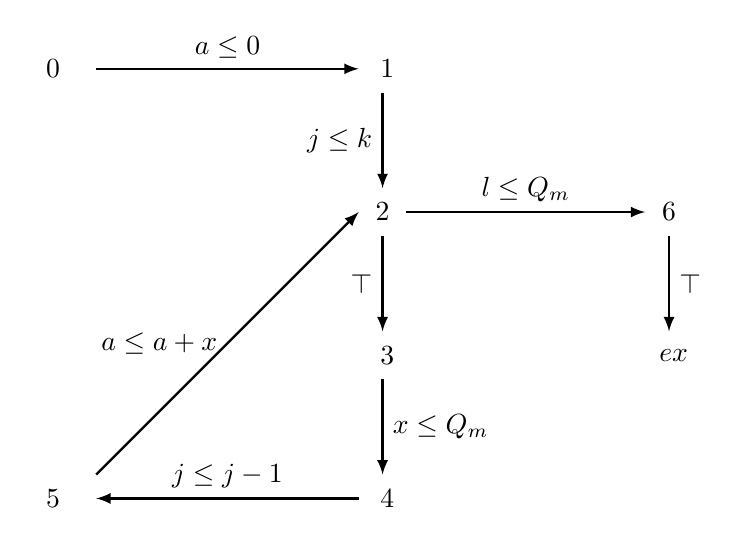
\begin{tikzpicture}[scale=\textwidth/20cm,samples=200]
  \draw[] (-7, 10) circle (0pt) node{{ $0$}};
  \draw[] (0, 10) circle (0pt) node{{ $1$}};
  \draw[] (0, 7) circle (0pt) node{\textbf{$2$}};
  \draw[] (0, 4) circle (0pt) node{{ $3$}};
  \draw[] (0, 1) circle (0pt) node{{ $4$}};
  \draw[] (-7, 1) circle (0pt) node{{ $5$}};
  % Counter Variables
  \draw[] (6, 7) circle (0pt) node {\textbf{$6$}};
  \draw[] (6, 4) circle (0pt) node {{ $ex$}};
  %
  % Control Flow Edges:
  \draw[ thick, -latex] (-6, 10)  -- node [above] {$a \leq 0$}(-0.5, 10);
  \draw[ thick, -latex] (0, 9.5)  -- node [left] {$j \leq k$} (0, 7.5) ;
  \draw[ thick, -latex] (0, 6.5)  -- node [left] {$\top$}  (0, 4.5);
  \draw[ thick, -latex] (0, 3.5)  -- node [right] {$x \leq Q_m$} (0, 1.5) ;
  \draw[ thick, -latex] (-0.5, 1)  -- node [above] {$j \leq j - 1$} (-6, 1) ;
  \draw[ thick, -latex] (-6, 1.5)  -- node [left] {$a \leq a + x$} (-0.5, 7)  ;
  \draw[ thick, -latex] (0.5, 7)  -- node [above] {$l \leq Q_m$}  (5.5, 7);
  \draw[ thick, -latex] (6, 6.5)  -- node [right] {$\top$} (6, 4.5) ;
  \end{tikzpicture}
  \caption{}
    \end{centering}
    \end{subfigure}
    \begin{subfigure}{.45\textwidth}
      \begin{centering}
    %   \todo{abstract-cfg for two round}
    \begin{tikzpicture}[scale=\textwidth/20cm,samples=200]
    \draw[] (-10, 10) circle (0pt) node{{ $0: 1$}};
    \draw[] (0, 10) circle (0pt) node{{ $1: 1$}};
    \draw[] (0, 7) circle (0pt) node{\textbf{$2: k$}};
    \draw[] (0, 4) circle (0pt) node{{ $3: k$}};
    \draw[] (0, 1) circle (0pt) node{{ $4: k$}};
    \draw[] (-10, 1) circle (0pt) node{{ $5: k$}};
    % Counter Variables
    \draw[] (6, 7) circle (0pt) node {\textbf{$6: 1$}};
    \draw[] (6, 4) circle (0pt) node {{ $ex: 1$}};
    %
    % Control Flow Edges:
  \draw[ thick, -latex] (-8, 10)  -- node [above] {$a \leq 0$}(-1.5, 10);
  \draw[ thick, -latex] (0, 9.5)  -- node [left] {$j \leq k$} (0, 7.5) ;
  \draw[ thick, -latex] (0, 6.5)  -- node [left] {$\top$}  (0, 4.5);
  \draw[ thick, -latex] (0, 3.5)  -- node [right] {$x \leq Q_m$} (0, 1.5) ;
  \draw[ thick, -latex] (-1.5, 1)  -- node [above] {$j \leq j - 1$} (-8, 1) ;
  \draw[ thick, -latex] (-8, 1.5)  -- node [left] {$a \leq a + x$} (-1.5, 7)  ;
  \draw[ thick, -latex] (1.5, 7)  -- node [above] {$l \leq Q_m$}  (4.5, 7);
  \draw[ thick, -latex] (6, 6.5)  -- node [right] {$\top$} (6, 4.5) ;
    \end{tikzpicture}
    \caption{}
      \end{centering}
      \end{subfigure}
    \caption{(a) The same $\kw{towRounds(k)}$ program as Figure~\ref{fig:twoRounds_example}
    (b) The abstract control flow graph for $\kw{towRounds(k)}$  (c) The abstract control flow graph with the reachability bound for $\kw{towRounds(k)}$.}
    \vspace{-0.5cm}
    \label{fig:abscfg_tworound}
  \end{figure}
\end{example}

%
% In order to estimate weight for every vertex in $\progV(c)$,
%  I first show how to compute the reachability bound for every label in $c$
%  % (i.e., every vertex in $\absV(c)$)
%  (i.e., the $\absW(c)$), 
%  then show how to compute the weight for every vertex in $\progV(c)$.
%  \\
%  Through the edges in $\absG(c)$, which correspond to $c$'s abstract transition between labels,

%  \wq{In order to estimate weight for every vertex in the static analysis dependency graph($\progV(c)$), I want to find out the upper bound on 
%  the number of times the labeled command (uniquely associated with a vertex in $\progV(c)$) may be executed when running the program.
%  This information can be obtained by computing the reachability bound for every vertice in the abstract control flow graph ($\absW(c)$), because
%  the vertices in the two graph share the same unique label, the line number.  I can easily show that the reachability bound on one vertex of the actract control flow graph is also the upper bound for the corresponding vertex in the static analysis dependency graph, both vertices share the same unique line number.}



%   I perform the symbolic reachability bound anaysis on the abstract control flow graph, 
%  through the edges in $\absG(c)$, which correspond to $c$'s abstract transition between labels.
%  I infer the invariant for every variable, and compute the transition closure for every abstract transition. By solving the closure
%  with the invariants of variables involved in this closure for every transition, I compute
%  the symbolic reachability bound of every commands corresponding to this transition.
%  \\
%  Specifically in four steps, Variable Modification Tracking, Local Bounds Computation,
%  the symbolic reachability bound of every commands corresponding to this transition. Specifically, this analysis can be performed in four steps:
%   Variable Modification Tracking, Local Bounds Computation,
%  Invariant Inference and Closure Generation, and Reachability Bound Computation,
\subsubsection{Reachability-Bound Analysis}
\label{sec:static-reachability}
\highlight{
  In order to estimate the data dependency quantity presented in Section~\ref{sec:dynamic-reachability},
% weight for every vertex in the static analysis dependency graph($\progV(c)$), 
it is necessary to find out the upper bound on
the number of times the labeled command
% (uniquely associated with a vertex in $\progV(c)$)
may be executed when running the program precisely and efficiently.
}
This information can be obtained by computing the reachability bound for every vertex in the abstract control flow graph ($\absW(c)$), because
the vertices in the two graph share the same unique label, the line number. 
This analysis is sound in the sense that
the reachability bound on one vertex of the abstract control flow graph is also the upper bound for
the corresponding dependency quantity of the labeled variable through the execution-based analysis in Section~\ref{sec:dynamic-reachability}.
% vertex in the static analysis dependency graph, both vertices share the same unique line number.

The symbolic reachability bound analysis is performed on the abstract control flow graph generated above.
The analysis is summarized as follows. 
% Through the edges in $\absG(c)$, which correspond to $c$'s abstract transition between labels.
I infer the invariant for every variable, and compute the transition closure for every abstract transition. By solving the closure
with the invariants of variables involved in this closure for every transition, I compute
the symbolic reachability bound of every commands corresponding to this transition. Specifically, this analysis can be performed in four steps:
 Variable Modification Tracking, Local Bounds Computation,
Invariant Inference and Closure Generation, and Reachability Bound Computation,
% 
%  I present the details of invariant, closure generation, and reachability bound computation as follows.
with details as follows.
%
%
\paragraph*{Variable Modification Tracking}
Identify the abstract events where each variable is increased, decreased and reset:
\\
$\inc: \mathcal{VAR} \to \mathcal{P}(\absevent) $
the set of the abstract events where the variable increase.
\\
$\inc(x) = \{(\absevent, c) | \absevent = (l, l', x' \leq x + v)\}$
\\
$\reset: \mathcal{VAR} \to \mathcal{P}(\absevent) $
The set of the abstract events where the variable is reset.
\\
$\dec: \mathcal{VAR} \to \mathcal{P}(\absevent) $
The set of abstract events where the variable decrease.
% \\
% $\dec(x) = \{(\absevent, c) | \absevent = (l, l', x' \leq x - v)\}$
\\
$Incr(v) \triangleq \sum\limits_{(\absevent, c) \in \inc(v)}\{\absclr(\absevent) \times v\}$
%
\paragraph*{Local Bounds}
Given a program $c$ with its abstract control flow graph 
$\absG(c) = (\absV, \absE)$
\\
Local Bounds Computation:
$\locbound: \absevent \to \mathcal{VAR} \cup \constdom$.
%
\[ 
\begin{array}{ll}
  \locbound(\absevent) \triangleq 1 
  & \absevent \notin SCC(\absG(c))
  \\
  \locbound(\absevent) \triangleq (x, v) 
  & \absevent \in SCC(\absG(c)) \land \absevent \in \dec(x) \land  \absevent = (\_, \_ , x' \leq x - v) \\
  \locbound(\absevent) \triangleq (x, \max(\dec(x))) 
  & \absevent \in SCC(\absG(c)) \land 
  \absevent  \notin \bigcup_{x \in \mathcal{VAR}} \dec(x)
  \land \absevent \notin SCC(\absG(c) \setminus \dec(x)) 
\end{array}
  \]
  The first case is straightforward. Since variable's visiting time outside of any while loop is at most 1, I do not need to analyze the visiting times of every node in the graph from phase 1.
  The second and third step is guaranteed by the \emph{Discussion on Soundness} in Section 4 of \cite{sinn2017complexity}.
  Then soundness proof is in Lemma~\ref{lem:local_bound_sound} in Appendix~\ref{apdx:reachability_soundness}.
%
\paragraph*{Invariant Inference and Closure Generation }
Then, computing the bound invariants for variables and the transition closures for abstract events:
\\ 
$ \varinvar: \mathcal{VAR} \cup \constdom \to EXPR(\constdom)$
\\
$\absclr: \absevent \to EXPR(\constdom)$
\\
Then, the symbolic invariant for each variable 
as well as the symbolic transition closure for each transition is calculated as follows:
\[ 
\begin{array}{lll}
  \varinvar(x) & \triangleq c & c \in \constdom \\
  \varinvar(x) & \triangleq Incr(v) + \max(\{\varinvar(a) + c | (t, a, c) \in \reset(x)\}) & c \notin \constdom
\end{array}
\]
%
\begin{defn}
  \label{def:transition_closure_base}
\[ 
\begin{array}{lll}
  \absclr(\absevent) 
  & \triangleq x / v & \\ 
  & \locbound(\absevent) = (x, v) \in \constdom \times \mathbb{N} & \\
  \absclr(\absevent) 
  & \triangleq (Incr(x) + 
  \sum\limits_{(\absevent', y, v') \in \reset(x)}
  \absclr(\absevent') \times \max(\varinvar(y) + v', 0) ) / v & \\
  & \locbound(\absevent) = (x, v) \land x \notin \constdom & 
\end{array}
  \]
\end{defn}
%
\paragraph*{Improved Variable Modification Tracking}
Instead of just identifying the abstract events where each variable is reset,
this improvement identifies the chain of the events where a given variable is reset by the 
variables of the abstract events through the chain.
\\
$\resetchain: \mathcal{VAR} \to \mathcal{P}(\mathcal{P}(\absevent)) $
The set of the chain of abstract events where the variable is reset through the chain.
% \\
% $Incr(v) \triangleq \sum\limits_{(\absevent, c) \in \inc(v)}\{\absclr(\absevent) \times v\}$
%
\paragraph*{Improved Invariant Inference and Closure Generation}
Then, computing the bound invariants for variables and the transition closures for abstract events:
\\ 
$ \varinvar: \mathcal{VAR} \cup \constdom \to EXPR(\constdom)$
\\
$\absclr: \absevent \to EXPR(\constdom)$
\\
Then, the symbolic invariant for each variable 
as well as the symbolic transition closure for each transition is calculated as follows:
\[ 
\begin{array}{lll}
  \varinvar(x) & \triangleq c & c \in \constdom \\
  \varinvar(x) & \triangleq Incr(v) + \max(\{\varinvar(a) + c | (t, a, c) \in \reset(x)\}) & c \notin \constdom
\end{array}
\]
%
\begin{defn}
  \label{def:transition_closure}
\[ 
\begin{array}{lll}
  \absclr(\absevent) 
  & \triangleq x / v & \\ 
  & \locbound(\absevent) = (x, v) \in \constdom \times \mathbb{N} & \\
  \absclr(\absevent) 
  & \triangleq \Big(
    \sum\limits_{y \in \{ y ~|~ 
    ch \in \resetchain(x), (l_1, x, y, v, l_2) \in ch \} } Incr(x) & \\
    & \quad + 
  \sum\limits_{ch \in \resetchain(x)}
  \big( \min\limits_{\absevent' \in ch}({\absclr(\absevent')}) \times 
  \max(\varinvar(y) + \sum\limits_{(l_1, x, y, v, l_2) \in ch } v, 0)\big) \Big) / v & \\
  & \locbound(\absevent) = (x, v) \land x \notin \constdom & 
\end{array}
  \]
\end{defn}
  %
% \paragraph*{Adding the Reachability Bounds for Every Vertex in the Data-Control Flow Graph}
% Updating the weight of every vertex in the $\progG(c) = (\progV, \progE, \progW, \progF)$ for program $c$ generated from phase 1. 
% For every $x^l \in \progV$, find the abstract event $\absevent \in \absflow(c)$ of the form $(l, \_, \_)$, updating the $\progW(x^l) $ by the transition closure of this event.
% \\
$
\progW(x^l) 
  \triangleq \absclr(\absevent)
$
\paragraph*{Reachability Bound Computation}
Through the transition closure computed above, 
The weight of every label in 
% Then I update 
the program $c$'s abstract control flow graph,
$\absG(c) =(\absV, \absE, \absW)$
is 
computed as the maximum over all the abstract events $\absevent \in \absE$ heading out from this vertex, formally as follows.
% by annotating each vertex with a symbolic weight. 
% This weight corresponds to 
%reachability bounds of
\\
$\absW 
\triangleq \left\{ (l, w) \in \mathbb{N} \times EXPR(\constdom) | w = \max\limits_{\absevent = (l, \_, \_)} \{ \absclr(\absevent)\} \right\}$.
% \\
\paragraph*{Example}
 I perform the symbolic reachability bound analysis on the abstract control flow graph as follows. 
 I would like to generate the closure of every edge, which is an equality relation between variables.  Solving this closure gives us the reachability bound for this edge. With all the bound for all the edges in the abstract control flow graph, I can calculate the weight for every vertex in this graph. For example, I show the closure generated for the edge 
$(4, j < j - 1, 5)$, 
$\absclr(4, 5) = \varinvar(j)$. The invariant for variable $j$, $\varinvar(j)$ used here is 
$\varinvar(j) = k * \absclr(1, 2)$, which is generated by all the difference constraints involving $j$ in the graph. Notice the $k$ in $\varinvar(j)$ comes from considering both difference constraint $j<=k$ from edge (1,2) and $j<=j-1$ from (4,5), which intuitively reflects the while loop whose counter is set to $k$ at the beginning and decreases by 1 at each iteration. 
With all the closures for all the edges of the abstract control flow graph, I can solve them to obtains the reachability bound of every edge.  I decide the weight for every vertex in the abstract control flow graph by using the bound of the edges which head out from this vertex, by taking the max of the bound from these involving edges. For instance,   
By the constraint on the edge $(4, j \leq j - 1, 5)$, I get bound $k$ for this edge.
Then, I assign vertex $4$ by reachability bound $k$, as in Figure~\ref{fig:abscfg_tworound}(c). 
Another interesting vertex is $2$, which has more than one edge heading out from it, $(2, \top, 3)$ and $(2,\top, 6)$. For the weight for vertex $2$, I choose the max between the bound $k$ from $(2,\top, 3)$ and $1$ from $(2,\top, 6)$.
The same way for the rest weights' computation.
 I use $\absW(c)$ for the set of weights I just computed 
for each label in the abstract control flow graph of $c$.
% Still looking at the two-round example as in Figure~\ref{fig:adapfun_tworound}(b) where 
% each label $l$ is added with a weight by $absW$.
% This weight represents the  maximum reaching times of this location $l$, in the other word, 
% the estimated maximum visiting times of the command labeled with $l$.
% For example, looking at the vertex $1$,
% by analysis steps, since it isn't in any SCC, it's estimated reachability bound is computed as $1$.
% However, for the vertex $4$ which is involved in an SCC, the reachability bound is inferred in another way.
% By the constraint on the edge $4, j \leq j - 1, 5$,
% I first infer its local bound as variable $j$.
% Then by solving the invariant for variable $j$,
% I infer the value bound for $j$, which is $k$.
% Then the reachability bound for this abstract transition, (i.e., edge $4, j \leq j - 1, 5$) 
% is computed as $k$ as well through Definition~\ref{def:abs_trace}.
% In this abstract control flow graph, every vertex is a label,
% corresponding to a label command in the program.
% Each directed 
% edge represents an abstract transition 
% between two control locations, 
% i.e., the labels of two commands (we call the labels also control location and they refer to the same thing), 
% where the second labeled command will be executed after execution of the command with first label.
% For example, the edge $0, a \leq 0, 1$ on the top, represents,
% from location $0$, the command 
% $\clabel{\assign{a}{0}}^0$ is executed with next continuation location $1$,
% where the 
% command $\clabel{\assign{j}{k}}^1$ will be executed next.
% The constraint $a \leq 0$ is generated by abstracting from the assignment command $\assign{a}{0}$,
% representing that value of $a$ is less than or equals to $0$ after 
% location $0$ before executing command at line $1$.
%
The same way for the rest weights' computation.
% \paragraph{Vertex Weight Computation}
% % The weight for each vertex in $\progV(c)$ is computed as follows,
% Then I compute the weight for each vertex in $\progV(c)$,
% % as a set of pairs $\progW(c) \in \mathcal{P}(\mathcal{LV} \times \mathcal{LV} \times EXPR(\constdom))$ 
% as a set of pairs 
% % is the set of pairs 
% % The weight for each vertex in $\progV(c)$ is computed 
% mapping each $x^l \in \progV(c)$ to a symbolic expression over $\constdom$. Since symbolic expression 
% over $\constdom$ is a subset of arithmetic expressions,
% we use $\mathcal{A}_{in}$ denotes the arithmetic expression 
% over $\mathcal{N}$ and input variable and $\progW(c) \in \mathcal{P}(\mathcal{LV} \times \mathcal{A}_{in})$ 
% as follows,
% \highlight{
% % :
% % \\
%  \[\progW(c) \triangleq
%    \left\{ (x^l, w) 
%   %  \in  \mathcal{LV} \times \expr
% \mid
% x^l \in \progV(c) \land (l, w) \in \absW(c)
% \right\}.
% \]
% }
% %
% % Since 
%  I prove that this 
% % symbolic expression is the upper bound for $x^l$'s 
% symbolic expression for $x^l \in \progV(c)$ is a sound upper bound of 
% the weight for the same vertex $x^l$ in Program's execution-based dependency graph in Appendix~\ref{apdx:reachability_soundness}.
% The maximum visiting times of $x^l$ over all execution traces of $c$ in Appendix~\ref{apdx:reachability_soundness}. 
% %
% \begin{thm}[Soundness of the Reachability Bounds Estimation]
%   \label{thm:addweight_soundness}
% Given a program ${c}$ with its program-based dependency graph 
% $\progG = (\progV, \progE, \progW, \progF)$,
% $\traceG = (\traceV, \traceE, \traceW, \traceF)$, I have:
% %
% \[
% \forall (x^l, w_{t}) \in \traceW,
% (x^l, w_{p}) \in \progW, \vtrace \in \mathcal{T} \sthat 
% % \lvar_c \sthat  
% %  \vcounter(\vtrace') l ~ \middle\vert~
% % \forall \vtrace \in \mathcal{T} \sthat  
% \config{{c}, \trace} \to^{*} \config{\eskip, \trace\tracecat\vtrace'} 
% \land 
% \config{w_{p}, \trace} \earrow v
% \implies
% % \right\} 
% \leq 
% w_{t}(\trace) \leq v
% \]
% \end{thm}
% \paragraph*{Example}
% Now let's 
% % where I goes 
% go back to the Program-Based Dependency Graph which I aim to build for approximating the 
% Execution-Based Dependency graph for two-round example, as in
% Figure~\ref{fig:twoRounds_example}(c).
% %
% %  looking at the two-round example,
% %  as in  where we
% % each vertex in 
% %  $l$ is added with a weight by $absW$.
% % This weight represents the  maximum reaching times of this location $l$, in the other word, 
% % the estimated maximum visiting times of the command labeled with $l$.
% % For example, looking at the vertex $1$,
% % by analysis steps, since it isn't in any SCC, it's estimated reachability bound is computed as $1$.
% % However, for the vertex $4$ which is involved in an SCC, the reachability bound is inferred in another way.
% % By the constraint on the edge $4, j \leq j - 1, 5$,
% % I first infer its local bound as variable $j$.
% % Then by solving the invariant for variable $j$,
% Every vertex from $\progV(c)$ in this graph corresponds to a labeled variable, for example $a^5$,
% and this label $5$ is also a vertex $5$ in the abstract control flow graph in Figure~\ref{fig:abscfg_tworound}(b).
% %
% % I infer the value bound for $j$, which is $k$.
% % Then the reachability bound for this abstract transition, (i.e., edge $4, j \leq j - 1, 5$) 
% Then, it is straight forward, 
% that the reachability bound for the label $5$, 
% is also the maximum visiting times bound of the labeled variable $a^5$.
% % is computed as $k$ as well through Definition~\ref{def:abs_trace}.
% % In this abstract control flow graph, every vertex is a label,
% % corresponding to a label command in the program.
% So, I estimate the visiting time for  labeled variable $a^5$ in Program-Based Dependency Graph in Figrue~\ref{fig:abscfg_tworound}(c) as $k$ as well.
% %
% The same way for the rest weights' computation.
% %
% \paragraph*{Data Dependency Quantity over pair of Labeled Variables }
% Then we define the estimated directed edges
% % for each vertex in $\progV(c)$,
% between vertices $({x}_1^{i}, w_1)$  
% and $({x}_2^{j}, w_2)$ 
% where ${x}_1^{i}, {x}_2^{j} \in \lvar(c)$,
% as a set of triples 
% % $\progW(c) \in \mathcal{P}(\mathcal{LV} \times \mathcal{LV} \times EXPR(\constdom))$ 
% $\progE(c) \in \mathcal{P}(\mathcal{LV} \times \mathcal{A}_{\lin} \times \mathcal{LV})$
% % is the set of pairs 
% % The weight for each vertex in $\progV(c)$ is computed 
% indicating a directed edge from the first vertex to the second one in each pair
% as follows,
% \highlight{
%   \[
%     \progE^0(c) \triangleq 
%     \left\{ 
%     ({x}_1^{i}, w, {x}_2^{j}) \in \mathcal{LV} \times 
%     \mathcal{A}_{\kw{in}} \times \mathcal{LV}
%     ~ \middle\vert ~
%     \begin{array}{l}
%       {x}_1^{i}, {x}_2^{j} \in \lvar(c)
%     \land
%       % \\
%       \exists n \in \mathbb{N}, z_1^{r_1}, \cdots, z_n^{r_n} \in \lvar_{{c}} \sthat 
%       n \geq 0 \land
%       \\
%       \flowsto(x^i,  z_1^{r_1}, c) 
%       \land \cdots \land \flowsto(z_n^{r_n}, y^j, c) 
%     \end{array}
%     \right\}
%     \]
% }
% with compute the weight for each edge in $\progE(c)$ computed above,
% % % as a set of pairs $\progW(c) \in \mathcal{P}(\mathcal{LV} \times \mathcal{LV} \times EXPR(\constdom))$ 
% % as a set of pairs 
% % % is the set of pairs 
% % % The weight for each vertex in $\progV(c)$ is computed 
% % mapping each $x^l \in \progV(c)$ to a symbolic expression over $\constdom$. Since symbolic expression 
% % over $\constdom$ is a subset of arithmetic expressions,
% % we use $\mathcal{A}_{in}$ denotes the arithmetic expression 
% % over $\mathcal{N}$ and input variable and $\progW(c) \in \mathcal{P}(\mathcal{LV} \times \mathcal{A}_{in})$ 
% % as follows,
% \highlight{
% % :
% % \\
%  \[
%    \progE(c) \triangleq
%    \left\{ (x^i, w, y^j) 
% \mid
% (x^i, w, y^j) \in \progE^0(c) \land 
% % w = \max\limits_{\absevent = (i, \_, j)} \{ \absclr(\absevent)\} 
% w = \max \left\{ \absclr(\absevent) ~\mid~ \absevent \in \absflow(c) \land \absevent = (i, \_, j) \right\} 
% \right\}.
% \]
% }
% %
% % Since 
% We prove that this 
% % symbolic expression is the upper bound for $x^l$'s 
% symbolic expression $w$ for edge $(x^i, w, y^j) \in \progE(c)$
%  is a sound upper bound of 
% the weight for the same edge $(x^i, w', y^j)$ in Program's execution-based dependency graph in Appendix~\ref{apdx:edgeweight_soundness}.
% % The maximum visiting times of $x^l$ over all execution traces of $c$ in Appendix~\ref{apdx:reachability_soundness}. 
% %
% \begin{thm}[Soundness of the Edge Weight Estimation]
%   \label{thm:edgeweight_soundness}
% Given a program ${c}$ with its program-based dependency graph 
% $\progG = (\progV, \progE)$,
% $\traceG = (\traceV, \traceE)$, we have:
% %
% \[
% \forall (x^l, w_{t}) \in \traceW,
% (x^l, w_{p}) \in \progW, \vtrace \in \mathcal{T} \sthat
% \config{{c}, \trace} \to^{*} \config{\eskip, \trace_0 \tracecat \vtrace'} 
% \land 
% \config{w_{p}, \trace} \earrow v
% \implies
% % \right\} 
% \leq 
% w_{t}(\trace) \leq v
% \]
% \end{thm}
\subsubsection{The Dependency Quantity Estimation for Labeled Variables}
\label{sec:static-quantity-node}
% The weight for each vertex in $\progV(c)$ is computed as follows,
\highlight{
  The dependency quantity for every labeled variable $x^l \in \lvar(c)$ is estimated as the reachabilility-bound for the location of the same label
from the $\absW(c)$.
\\
As introduced in third step of this analysis framework in Section~\ref{sec:static-overview},
this information will be used in constructing the program-based dependency graph, to estimate the execution-based dependency graph for the program.
For easy understanding,
I reveal the
vertex and weight construction of this estimated graph below and presents the formal definition later. 
% In order to estimate the execution-based dependency graph for the program.
\\
% Then we compute the weight for each vertex in $\progV(c)$,
This weighted vertex set $\progV(c)$ is defined
% as a set of pairs $\progW(c) \in \mathcal{P}(\mathcal{LV} \times \mathcal{LV} \times EXPR(\constdom))$ 
as a set of pairs 
% is the set of pairs 
% The weight for each vertex in $\progV(c)$ is computed 
mapping each vertex $x^l \in \lvar(c)$ to a symbolic expression over $\constdom$,
$\progW(c) \in \mathcal{P}(\mathcal{LV} \times \mathcal{A}_{\lin})$, computed
as follows,
 \[\progV(c) \triangleq
   \left\{ (x^l, w) 
\mid
x^l \in \lvar(c) \land (l, w) \in \absW(c)
\right\}.
\]
}
%
% Since 
We prove that this 
% symbolic expression is the upper bound for $x^l$'s 
symbolic expression for $x^l \in \progV(c)$ is a sound upper bound of 
the weight for the same vertex $x^l$ in Program's execution-based dependency graph in Appendix~\ref{apdx:reachability_soundness}.
The maximum visiting times of $x^l$ over all execution traces of $c$ in Appendix~\ref{apdx:reachability_soundness}. 
%
\begin{thm}[Soundness of the Vertex Weight Estimation]
  \label{thm:vertexweight_soundness}
Given a program ${c}$ with its program-based dependency graph 
$\progG = (\progV, \progE)$,
$\traceG = (\traceV, \traceE)$, we have:
%
\[
  \begin{array}{l}
  \forall (x^l, w_{t}) \in \traceV,
  (x^l, w_{p}) \in \progV, 
  \trace_0 \in \mathcal{T}_0(c), 
  \trace' \in \mathcal{T}, v \in \mathbb{N} \sthat
  \\ \quad
  \config{{c}, \trace_0} \to^{*} \config{\eskip, \trace_0\tracecat\vtrace'} 
  \land 
  \config{w^{p}, \trace_0} \earrow v
  \implies
  % \right\} 
  w_{t}(\trace) \leq v
  \end{array}
\]
\end{thm}
\paragraph*{Example}
Now let's 
% where we goes 
go back to the Program-Based Dependency Graph which we aim to build for approximating the 
Execution-Based Dependency graph for two-round example, as in
Figure~\ref{fig:twoRounds_example}(c).
%
Every vertex from $\progV(c)$ in this graph corresponds to a labeled variable, for example $a^5$,
and this label $5$ is also a vertex $5$ in the abstract control flow graph in Figure~\ref{fig:abscfg_tworound}(b).
%
% we infer the value bound for $j$, which is $k$.
% Then the reachability bound for this abstract transition, (i.e., edge $4, j \leq j - 1, 5$) 
Then, it is straight forward, 
that the reachability bound for the label $5$, 
is also the maximum visiting times bound of the labeled variable $a^5$.
% is computed as $k$ as well through Definition~\ref{def:abs_trace}.
% In this abstract control flow graph, every vertex is a label,
% corresponding to a label command in the program.
So, we estimate the visiting time for  labeled variable $a^5$ in Program-Based Dependency Graph in Figrue~\ref{fig:abscfg_tworound}(c) as $k$ as well.
%
The same way for the rest weights' computation.
%
\subsubsection{The Dependency Quantity Estimation for the Pair of Labeled Variables}
\label{sec:static-quantity-edge}
The dependency quantity for every pair of labeled variables $x^i, y^j \in \lvar(c)$ is also estimated
as the minimum reachability-bounds of the locations having the same label $i, j$
from the $\absW(c)$.
\\
% Again, as introduced in third step of this analysis framework in Section~\ref{sec:static-overview}, we also build the
\highlight{
For the same reason in Section~\ref{sec:static-quantity-node},
I reveal the construction of
weight for every edge below with the formal definition presented later.
% In order to estimate the execution-based dependency graph for the program.
% The weight for each vertex in $\progV(c)$ is computed as follows,
The weight for each edge in $\progE(c)$ is computed as follows,
% % as a set of pairs $\progW(c) \in \mathcal{P}(\mathcal{LV} \times \mathcal{LV} \times EXPR(\constdom))$ 
% as a set of pairs 
% % is the set of pairs 
% % The weight for each vertex in $\progV(c)$ is computed 
% mapping each $x^l \in \progV(c)$ to a symbolic expression over $\constdom$. Since symbolic expression 
% over $\constdom$ is a subset of arithmetic expressions,
% we use $\mathcal{A}_{in}$ denotes the arithmetic expression 
% over $\mathcal{N}$ and input variable and $\progW(c) \in \mathcal{P}(\mathcal{LV} \times \mathcal{A}_{in})$ 
% as follows,
% :
% \\
 \[
   \progE(c) \triangleq
   \left\{ (x^i, w, y^j) 
\mid
(x^i, w, y^j) \in \progE^0(c) \land 
% w = \max\limits_{\absevent = (i, \_, j)} \{ \absclr(\absevent)\} 
w = \max \left\{ \absclr(\absevent) ~\mid~ \absevent \in \absflow(c) \land \absevent = (i, \_, j) \right\} 
\right\}.
\]
}
%
% Since 
We prove that this 
% symbolic expression is the upper bound for $x^l$'s 
symbolic expression $w$ for edge $(x^i, w, y^j) \in \progE(c)$
 is a sound upper bound of 
the weight for the same edge $(x^i, w', y^j)$ in Program's execution-based dependency graph in Appendix~\ref{apdx:reachability_soundness}.
% The maximum visiting times of $x^l$ over all execution traces of $c$ in Appendix~\ref{apdx:reachability_soundness}. 
%
\begin{thm}[Soundness of the Edge Weight Estimation]
  \label{thm:edgeweight_soundness}
Given a program ${c}$ with its program-based dependency graph 
$\progG = (\progV, \progE)$,
$\traceG = (\traceV, \traceE)$, we have:
%
\[
\forall (x^l, w_{t}) \in \traceW,
(x^l, w_{p}) \in \progW, \vtrace \in \mathcal{T} \sthat
\config{{c}, \trace} \to^{*} \config{\eskip, \trace_0 \tracecat \vtrace'} 
\land 
\config{w_{p}, \trace} \earrow v
\implies
% \right\} 
\leq 
w_{t}(\trace) \leq v
\]
\end{thm}
\paragraph*{Example}
Now let's 
% where we goes 
go back to the Program-Based Dependency Graph which we aim to build for approximating the 
Execution-Based Dependency graph for two-round example, as in
Figure~\ref{fig:twoRounds_example}(c).
Every edge is annotated by an arithmetic expression indicating the maximum number of executing time associating
the transition on this edge.

% \highlight{
%   \subsubsection{Improvements Analysis}
%   \label{sec:static-quantity-improvements}
% This new data dependency estimation algorithm is more precise and efficient than previous static analysis.
% % language and operational semantics design improves the expressiveness, efficiency, and the accuracy to a large extend.
% % \todo{Add details}
% \begin{itemize}
%   %   \item \textbf{Improvements on Expressiveness}
%   %   \\
%   % This language is extended over the standard while language. 
%   % In this sense, it supports all the general data analysis.
%   \item \textbf{Improvements on Efficiency}
%   \\
%   New analysis architecture does not rewrite the program into SSA version.
% \\
%   New analysis technique does not pre-collect the variables generated during the program.
% \\
%   New analysis technique does unfold the while loop and perform analysis for each iteration of the loop, 
%   instead, it only performs the analysis on the while body once.
%   \\
% In the three senses above, the efficiency is improved significantly.
%   \item \textbf{Improvements on Accuracy}
%   Comparing to previous dependency estimation method,
%   new analysis technique uses the reachable definition algorithm.
%   This algorithm improves the accuracy 
%   on the approximating the data dependency relation.
%   \end{itemize}
%   }